% kapitel4.tex
\chapter{Apl Waypoints Algorithmus}
\label{chapter:algorithmus3}
\graphicspath{{../bilder/}}

Der AplWaypoints-Algorithmus wurde entwickelt, um eine optimale Balance zwischen der durchschnittlichen Pfadlänge (Average Path Length, APL) und der maximalen Linkauslastung (Maximum Link Utilization, MLU) durch strategische Waypoint-Auswahl zu erreichen. Das Ziel ist ein robustes Netzwerk mit verteilter Auslastung bei gleichzeitig kurzen Pfaden für geringe Latenz.

\section{Zielfunktion und mathematische Grundlagen}

Die gewichtete durchschnittliche Pfadlänge wird berechnet als:
\[
\text{APL} = \frac{\sum_{(s,t,d) \in \mathcal{D}} d \cdot \text{dist}(s,t)}{\sum_{(s,t,d) \in \mathcal{D}} d}
\]

wobei $\mathcal{D}$ die Menge aller Demands $(s,t,d)$ mit Quelle $s$, Ziel $t$ und Demand-Größe $d$ darstellt, und $\text{dist}(s,t)$ die Hopanzahl des kürzesten Pfades zwischen $s$ und $t$ bezeichnet.

Der Algorithmus optimiert eine kombinierte Zielfunktion:
\[
\text{Objective} = \lambda \cdot \text{APL} + (1-\lambda) \cdot \text{MLU}
\]

wobei $\lambda \in [0,1]$ den Gewichtungsparameter darstellt. Für $\lambda = 0.5$ werden APL und MLU gleichgewichtet, für $\lambda < 0.5$ wird MLU priorisiert, und für $\lambda > 0.5$ wird APL stärker gewichtet.

\section{Zentralitätsbasierte Waypoint-Kandidatenauswahl}

Die Auswahl der Waypoint-Kandidaten basiert auf einem mehrdimensionalen Zentralitätsscore, der drei wesentliche Netzwerkmetriken kombiniert:
\[
\text{Score}(v) = \alpha \cdot \text{BC}(v) + \beta \cdot \text{DC}(v) + \gamma \cdot \text{DV}(v)
\]

wobei:
\begin{itemize}
    \item $\text{BC}(v)$ die normalisierte Betweenness Centrality von Knoten $v$ bezeichnet
    \item $\text{DC}(v)$ die Degree Centrality (Knotengrad) von Knoten $v$ darstellt
    \item $\text{DV}(v)$ das Demand-Volumen von Knoten $v$ repräsentiert
    \item $\alpha = 0.5$, $\beta = 0.3$, $\gamma = 0.15$ die empirisch bestimmten Gewichtungsparameter sind
\end{itemize}

Die Betweenness Centrality misst, wie häufig ein Knoten auf kürzesten Pfaden zwischen anderen Knotenpaaren liegt und identifiziert somit kritische Verbindungsknoten. Die Degree Centrality berücksichtigt die direkte Konnektivität eines Knotens, während das Demand-Volumen traffic-intensive Knoten ("Demand Hotspots") identifiziert.

\section{Kandidatenauswahl und Größenadaptivität}

Der Algorithmus wählt die $k$ besten Knoten basierend auf ihrem Zentralitätsscore als Waypoint-Kandidaten aus:
\[
  k = \max(10, \lfloor 0.2 \cdot |V| \rfloor)
\]

Diese adaptive Größenbestimmung ist bewusst gewählt: Für kleinere Topologien ($|V| < 50$) wird eine Mindestanzahl von $k = 10$ Kandidaten sichergestellt, um ausreichende Diversität zu gewährleisten. Bei größeren Topologien wird proportional $20\%$ der Knoten als Kandidaten betrachtet, um die Rechenkomplexität zu begrenzen und gleichzeitig eine repräsentative Auswahl zu erhalten.

\section{Demand-spezifische Waypoint-Optimierung}

Der Kernalgorithmus durchläuft alle Demands in absteigender Reihenfolge ihrer Demand-Größe. Für jede Demand $(s,t,d)$ wird systematisch evaluiert, welcher Waypoint-Kandidat $v$ den optimalen Pfad $s \rightarrow v \rightarrow t$ erzeugt.

Der Optimierungsprozess umfasst folgende Schritte:

\begin{enumerate}
    \item \textbf{Pfadberechnung}: Für jeden Kandidaten $v \in \mathcal{C}$ wird der kombinierte Pfad aus $\text{dist}(s,v) + \text{dist}(v,t)$ berechnet
    \item \textbf{Flow-Update}: Die Flüsse auf allen Links werden entsprechend der neuen Pfadführung aktualisiert:
    \begin{itemize}
        \item Entfernung des ursprünglichen Flusses auf dem direkten Pfad $s \rightarrow t$
        \item Addition des Flusses auf dem Waypoint-Pfad $s \rightarrow v \rightarrow t$
    \end{itemize}
    \item \textbf{Zielfunktionsberechnung}: Für jede Waypoint-Option wird die resultierende APL und MLU berechnet und die kombinierte Zielfunktion evaluiert
    \item \textbf{Beste Waypoint-Auswahl}: Der Waypoint mit der minimalen Zielfunktion wird für diese Demand ausgewählt
\end{enumerate}

\section{Globale Flow-Rekalkulation und Ergebnisvalidierung}

Nach der waypoint-spezifischen Optimierung aller Demands führt der Algorithmus eine globale Neuberechnung der Flows durch. Dies gewährleistet Konsistenz, da die sequenzielle Optimierung einzelner Demands zu suboptimalen Gesamtflüssen führen kann.

Die finale Lösung umfasst:
\begin{itemize}
    \item Eine Waypoint-Zuordnung für jede Demand in der Form ${d_{idx}: [(s,v), (v,t)]}$ für Waypoint-Pfade oder ${d_{idx}: [(s,t)]}$ für direkte Pfade
    \item Die resultierende MLU basierend auf den finalen Link-Auslastungen
    \item Die gewichtete APL unter Berücksichtigung aller gewählten Pfade
    \item Detaillierte Load-Informationen für jedes Link im Netzwerk
\end{itemize}

Der AplWaypoints-Algorithmus erzielt durch diese mehrstufige, zentralitätsbasierte Optimierung eine effektive Balance zwischen Pfadlängenminimierung und Lastverteilung, wodurch sowohl die Netzwerklatenz als auch die Auslastungseffizienz verbessert werden.

\section{Experimentelle Evaluation}
\label{sec:evaluation}

Zur Bewertung unseres Algorithmus testeten wir verschiedene Konfigurationen des $\lambda$-Parameters im Bereich $[0.0, 1.0]$ und analysierten den Trade-off zwischen der durchschnittlichen Pfadlänge (APL) und der maximalen Linkauslastung (MLU). 

Der entwickelte Algorithmus optimiert eine kombinierte Zielfunktion der Form $(\lambda \cdot \text{APL}) + (1-\lambda) \cdot \text{MLU}$, wobei $\lambda$ die Gewichtung zwischen beiden Metriken steuert. 

Abbildung~\ref{fig:pareto_apl_mlu} zeigt die resultierende Pareto-Front für verschiedene $\lambda$-Werte. Die Ergebnisse demonstrieren den erwarteten Zielkonflikt: Mit steigendem $\lambda$ sinkt die APL, während die MLU zunimmt.

\begin{figure}[htbp]
    \centering
    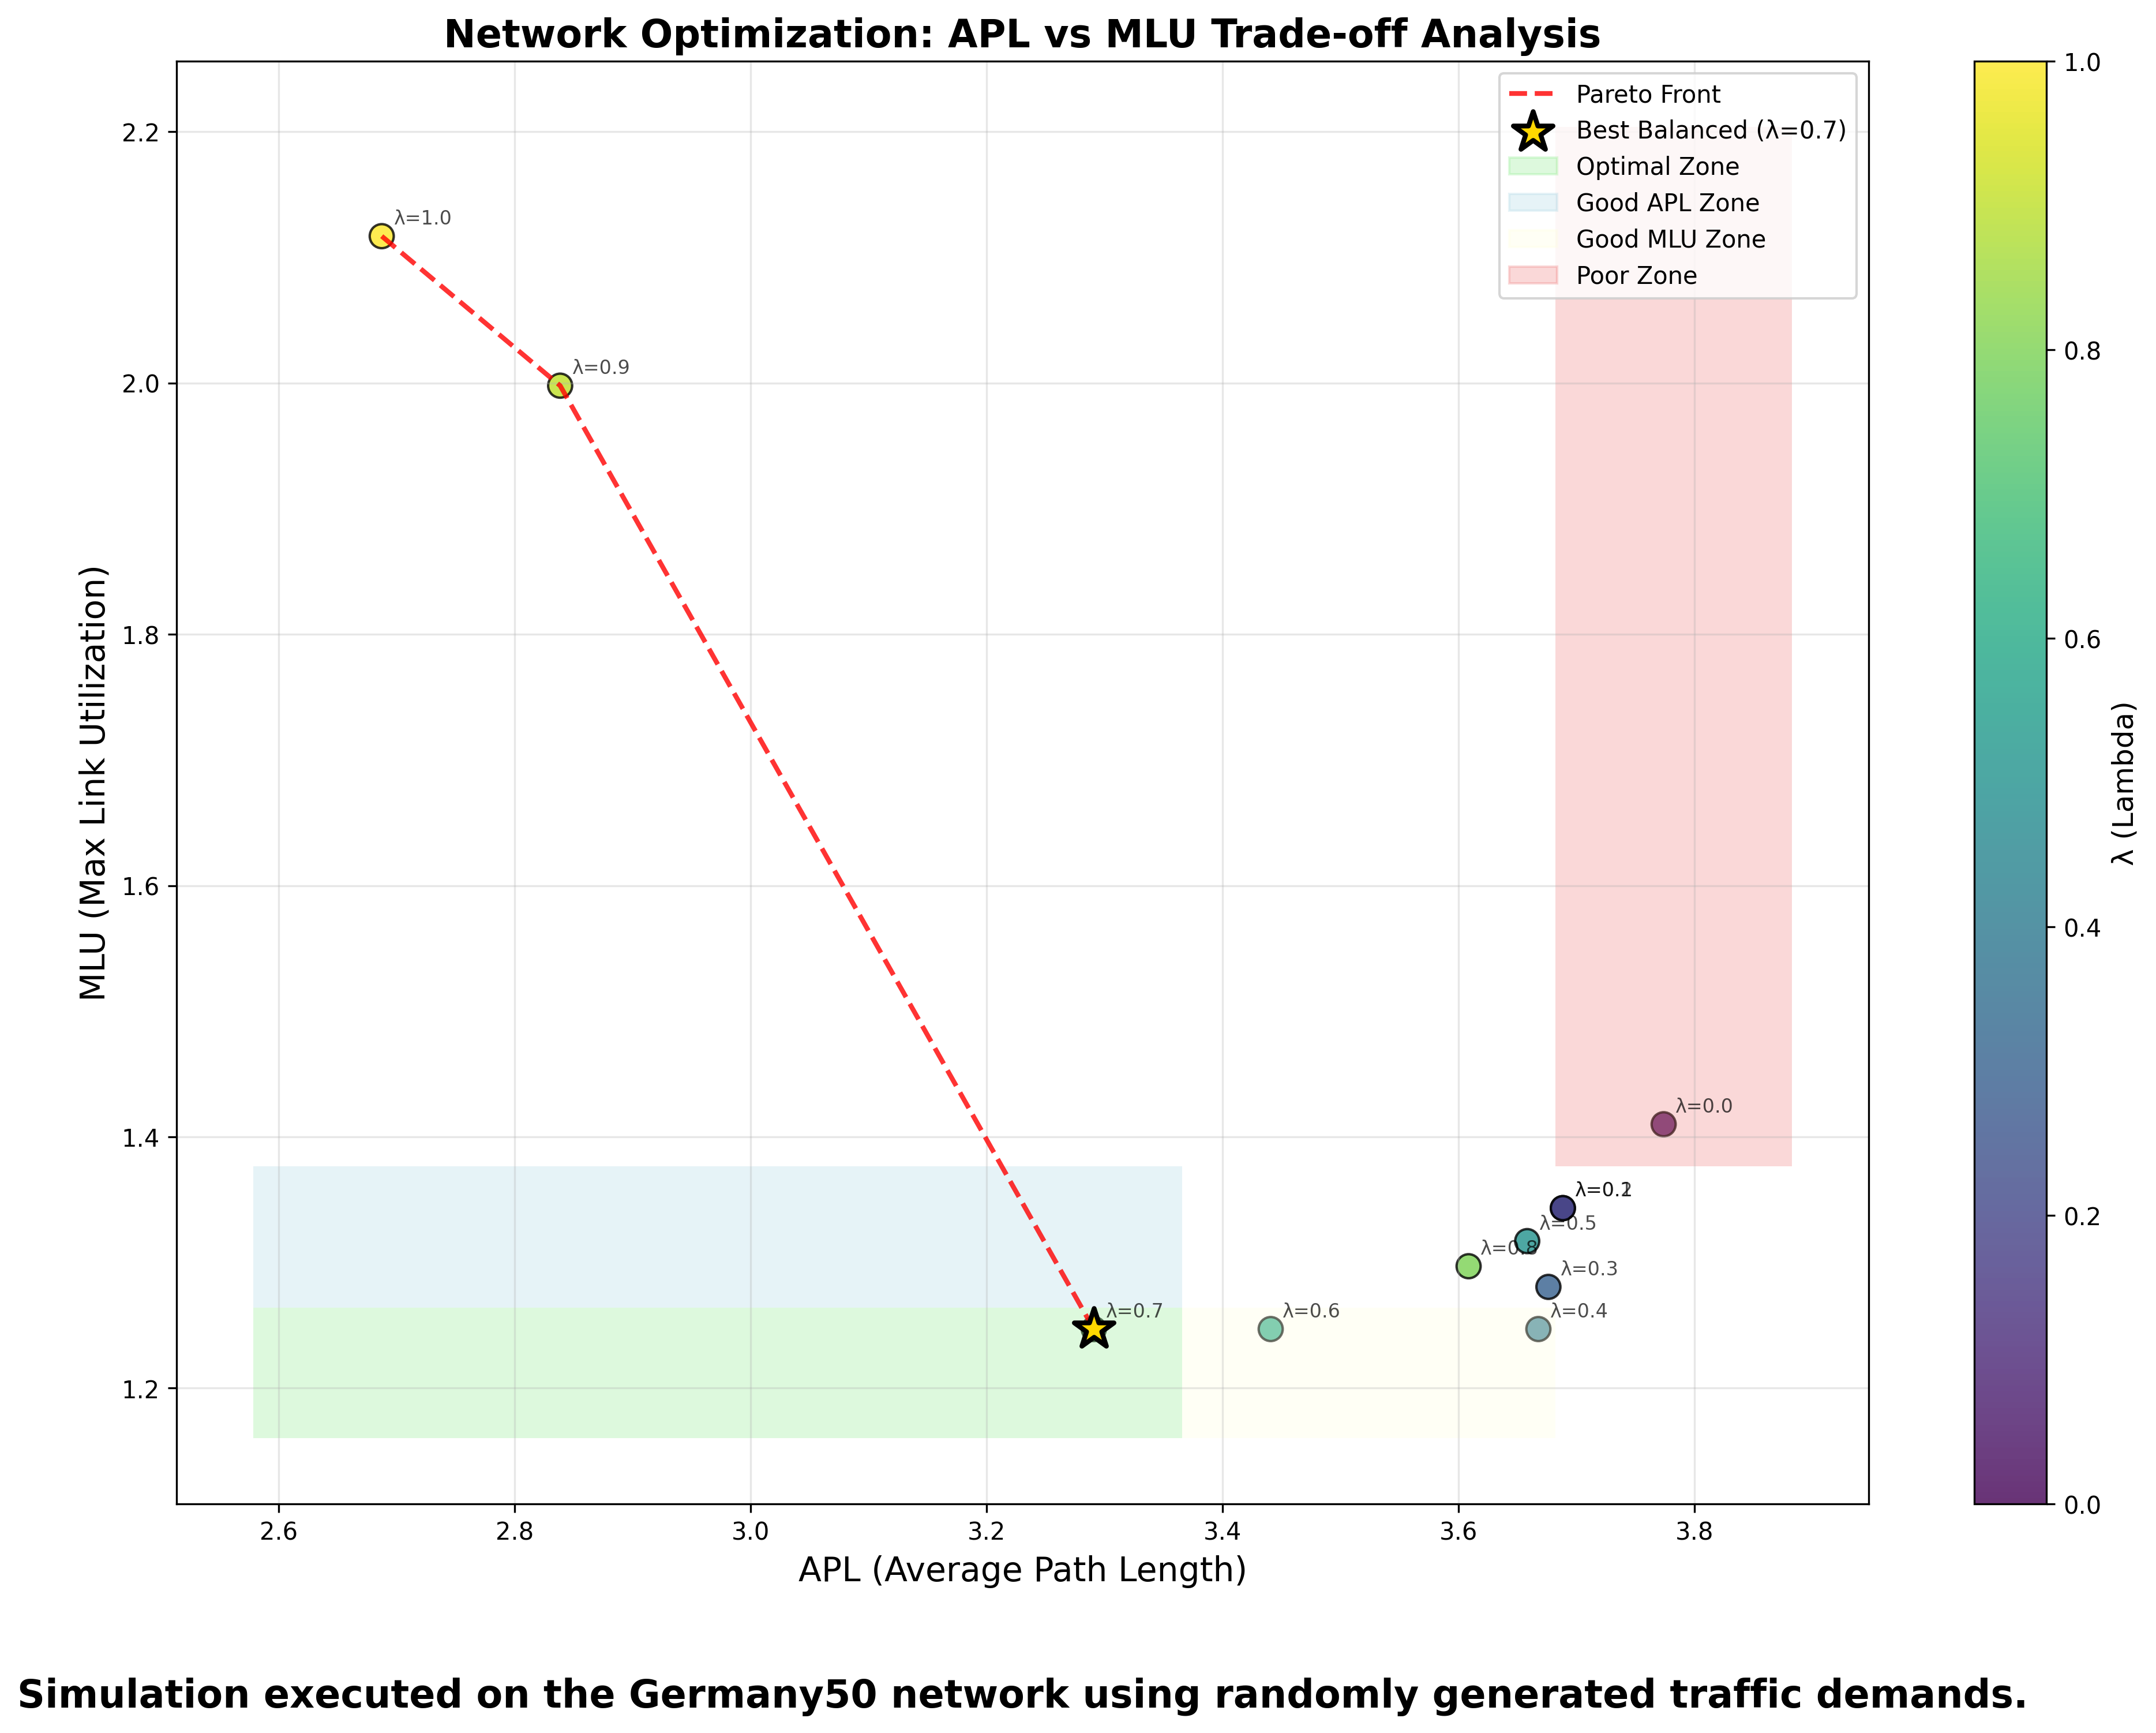
\includegraphics[width=0.8\textwidth]{DA-Vorlage/bilder/pareto_apl_mlu.png}
    \caption{Pareto-Front der APL-MLU-Optimierung für verschiedene $\lambda$-Werte. Der Punkt $\lambda = 0.7$ (markiert mit Stern) stellt einen ausbalancierten Kompromiss dar.}
    \label{fig:pareto_apl_mlu}
\end{figure}

Basierend auf dieser Analyse erweist sich insbesondere $\lambda = 0.3$ als praktikabler Wert, da er eine ausgewogene Lastverteilung bei akzeptabler Pfadlänge ermöglicht. Höhere Werte wie $\lambda = 0.7$ verbessern zwar die Latenz weiter, führen jedoch zu erhöhter Auslastung auf einzelnen Links. Die konkrete Wahl des optimalen Parameters sollte daher in Abhängigkeit der jeweiligen Netzwerkanforderungen (z.B. Verzögerung vs. Überlastresistenz) erfolgen.
\begin{figure}[htbp]
    \centering
    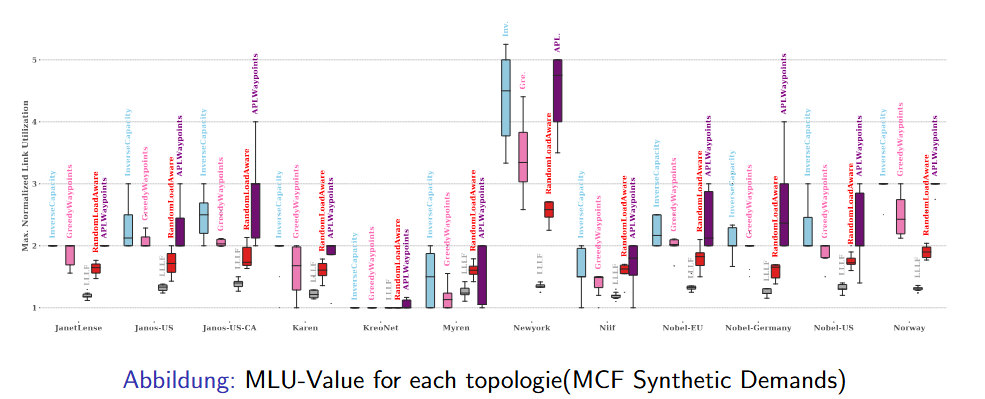
\includegraphics[width=0.95\textwidth]{DA-Vorlage/bilder/mlu_comparison.png}
    \caption{Vergleich der Maximum Link Utilization (MLU) verschiedener Routing-Algorithmen über mehrere Netzwerktopologien }
    \label{fig:mlu_synthetic}
\end{figure}

